\chapter*{Introduzione}
\addcontentsline{toc}{chapter}{Introduzione} \markboth{INTRODUZIONE}{}
Con la presente tesi si intende fornire una panoramica sulla bioinformatica, una delle scienze emergenti degli ultimi anni. L'obiettivo è quello di mostrare le applicazioni degli algoritmi alla biologia, in particolar modo lo studio e la costruzione degli \textit{alberi evolutivi}, che sono l'argomento principale.
\newline
Quest'ultimi, definiti anche \textit{alberi filogenetici}, sono una risorsa chiave sia nell'informatica che nella biologia in quanto permettono lo studio delle relazioni tra le entità biologiche e mostrano la loro evoluzione nel tempo.
\newline 
L'idea di base della struttura dei capitoli è quella di mostrare, innanzitutto, i concetti base di biologia, necessari per comprendere la materia in oggetto, dopodiché viene presentata la bioinformatica e le sue aree di ricerca, infine vengono illustrati gli algoritmi più importanti per la costruzione degli alberi evolutivi. Di seguito si mostra una panoramica di tali capitoli.
\begin{enumerate}
	\item \textit{Capitolo 1}: nozioni biologiche di base. Viene dato uno sguardo generale alla classificazione delle forme di vita, dai polisaccaridi fino agli acidi nucleici. Le sezioni successive mostrano il DNA, RNA e proteine. Tutti i concetti di questo capitolo sono funzionali alla comprensione della suddetta tesi. Senza di questi, infatti, non sarebbe possibile capire né contesto né senso di questo studio.
	\item \textit{Capitolo 2}: introduzione alla bioinformatica. Le sezioni successive, oltre a dare una definizione della materia e a raccontare la sua storia, dalla sua nascita fino ai giorni nostri, illustrano le principali aree di ricerca, dandone una breve spiegazione a ciascuna di essa.
	\newline
	Gli alberi evolutivi fanno parte della cosiddetta filogenetica, in quanto studia le relazioni evolutive tra le entità biologiche attraverso la costruzione di tali alberi.
	\item \textit{Capitolo 3}: viene mostrato l'albero evolutivo, cosa è, a cosa serve e che tipi di alberi si possono costruire. Si parla di albero radicato ed albero non radicato, entrambi con funzioni diverse, in quanto il primo mostra le evoluzioni delle entità biologiche, mentre il secondo mostra come sono legate tra loro. Tale capitolo svolge un ruolo chiave, in quanto vengono poste le basi per il capitolo successivo, che è il "cuore" della presenti tesi.
	\item \textit{Capitolo 4}: all'inizio di tale capitolo viene posto il problema che sta alla base degli alberi, ovvero il cosiddetto \textit{problema della costruzione degli alberi evolutivi}. Le sezioni successive mostrano come è possibile risolverlo: di volta in volta vengono mostrati algoritmi sempre più efficaci. Quindi si parte dall'idea di base, poi vengono evidenziate le criticità ed infine vengono sviluppati nuovi algoritmi volti a risolvere tali criticità. Il risultato finale di questa ricerca sono due algoritmi, il \textit{Neighbor-Joining} ed il \textit{Unweighted Pair Group Method with Arithmetic Mean (UPGMA)}, dove il primo permette la costruzione di alberi senza radice, mentre il secondo con radice.
	\newline
	Tutti gli algoritmi prendono in input una matrice $D$ definita \textit{matrice delle distanze}, in quanto ottenuta calcolando la distanza tra le coppie di elementi di cui è composta.
\end{enumerate}

\subsection*{Esempio di applicazione}
Perché gli alberi evolutivi sono così importanti? Perché grazie ad essi è possibile conoscere l'evoluzione delle specie e le relazioni tra le entità biologiche. Per entità non si intendono solamente gli animali o le piante, ma anche la classificazione di virus.
\newline
Nei primi anni duemila in Oriente, in particolar modo ad Hong Kong, in Cina, si è espansa a macchia d'olio una malattia infettiva, che nei casi più gravi si è rivelata fatale, ovvero la \textit{SARS} (Severe acute respiratory syndrome) che sta per "sindrome acuta respiratoria grave".
\newline
Gli scienziati hanno scoperto che questa malattia è causata da un virus chiamato Coronavirus, che attacca le vie aree sia degli animali che degli umani. All'inizio si era ipotizzato che il virus fosse stato trasmesso agli umani da parte di alcune specie di animali. Ma quali sono questi animali e come è stato possibile?
\newline
Attraverso la costruzione dell'albero evolutivo del Coronavirus è stato individuato il responsabile della trasmissione. Nello specifico sono state confrontate le sequenze del virus presente negli animali con quelle degli umani. La corrispondenza migliore è stata ottenuta con la civetta delle palme, un piccolo mammifero dalle fattezze simile all'ermellino. Gli scienziati suppongono che la trasmissione è avvenuta a causa del fatto che in Cina la civetta viene cacciata come cibo. 
\newline
In conclusione, tale scoperta ha permesso uno studio più approfondito del virus, oltre ad aver ridotto la sua diffusione.

\newpage


\chapter{Capitolo 1: Concetti base di biologia}
La bioinformatica è una materia che tratta tanto l'informatica quanto la biologia, pertanto è necessario illustrarne gli argomenti più importanti, che verranno spiegati in modo funzionale allo scopo della presente tesi.
\newline
La \textit{biologia} è la scienza che studia la vita, dagli attori che ne fanno parte fino ai processi in cui essi sono coinvolti \cite{campbellBiology}. Poiché la vita sulla terra si estende dalle profondità del mare fino alla biosfera, si è reso necessario organizzarla in differenti ordini di grandezza. L'atomo è l'unità elementare che costituisce tutta la materia. Insiemi di atomi formano le molecole che, a loro volta combinandosi, formano le macromolecole. Insieme sono i costituenti delle cellule, le più piccole strutture classificabili come organismi viventi.
\newline
Ci sono quattro tipi di macromolecole essenziali per tutte le forme di vita:
\begin{itemize}
	\item \textit{Polisaccaridi}: macromolecole formate da aggregazioni di monosaccaridi, tra cui il fruttosio, il glucosio e così via. Sono riserve di energia pronta.
	\item \textit{Proteine}: svolgono una vasta gamma di funzioni all'interno degli organismi viventi, permettendo le reazioni metaboliche, la replicazione del DNA, la risposta agli stimoli e così via.
	\item \textit{Lipidi}: chiamati anche grassi, sono le riserve energetiche di deposito.
	\item \textit{Acidi nucleici}: DNA e RNA, contengono e trasportano l'informazione genetica.
\end{itemize}
Le sezioni successive del capitolo sono dedicate al DNA, RNA e proteine.
\newpage

\section{DNA}
Il \textit{DNA} o \textit{acido desossiribonucleico} è una macromolecola contenente il patrimonio genetico\footnote{Il patrimonio genetico contiene tutte le informazioni genetiche di un organismo.} degli esseri viventi \cite{campbellBiology}, dunque ne detiene l\?informazione ereditaria \cite{BiologySolomon}.
\newline
Porzioni specifiche di DNA contengono determinate informazioni, ad esempio il colore degli occhi, dei capelli e così via. Queste prendono il nome di \textit{gene} \cite{MolecularCellBiology}.
\newline
Di seguito viene illustrata un'immagine del DNA, insieme ad una breve descrizione.
\newline
\begin{figure}[h!]
	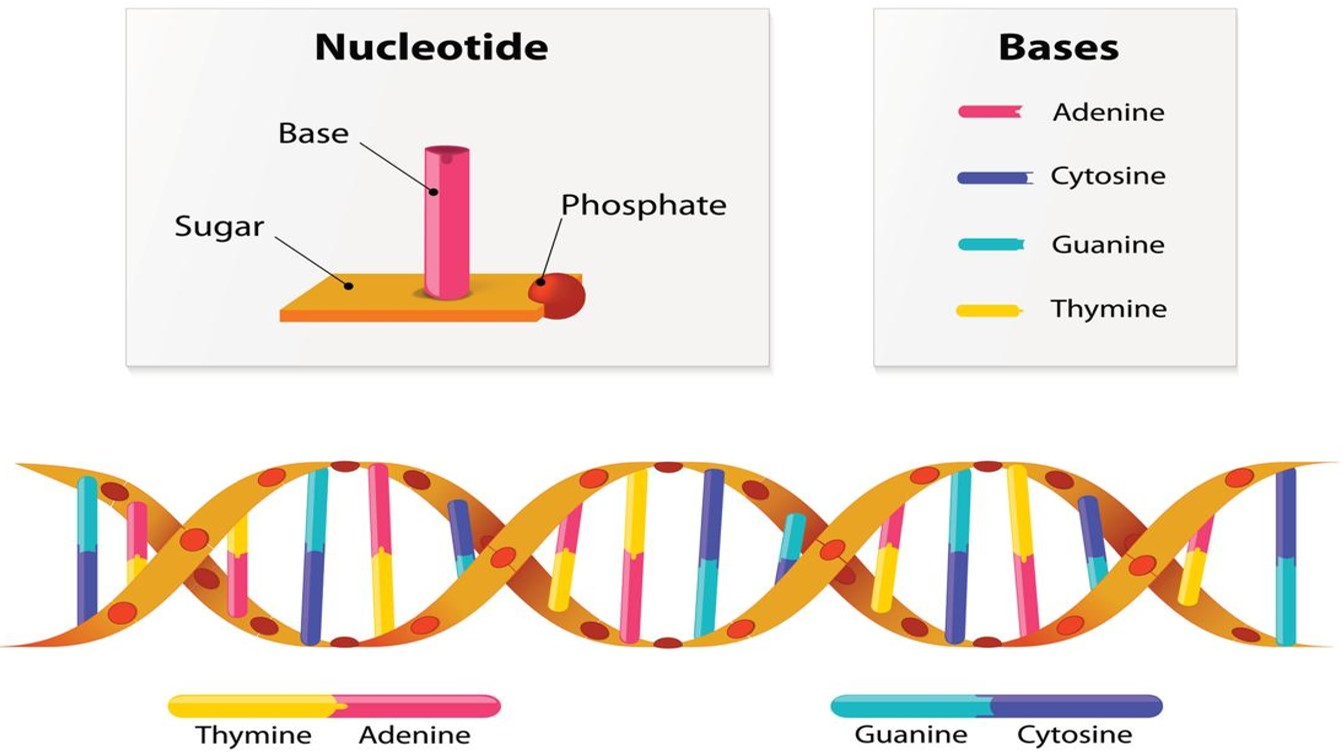
\includegraphics[width=\linewidth]{DNAStructure.jpg}
 	\caption{La struttura del DNA e del nucleotide.}
  	\label{fig:DnaAndNucleotideStructure}
\end{figure}
\newline
La struttura è caratterizzata da una doppia elica di lunghezza variabile, dove ciascun filamento è formato da una sequenza di molecole chiamate \textit{desossiribonucleotidi}.
\newline
Un desossiribonucleotide è composto da una molecola di zucchero, un gruppo fosfato ed una base azotata. Di quest'ultima, ne esistono quattro tipi:
\begin{itemize}
	\item \textit{adenina} (A);
	\item \textit{timina} (T);
	\item \textit{guanina} (G);
	\item \textit{citosina} (C).
\end{itemize}
Una proprietà importante delle basi azotate è che sono biunivocamente legate tra loro: l'Adenina si può legare solo con la Timina (A-T), mentre la Guanina con la Citosina (G-C). Questo significa che i filamenti sono complementari e quindi se conosciamo la sequenza di basi di un filamento di DNA sappiamo anche la sequenza di quello complementare.

\section{RNA}
L'\textit{RNA}, ovvero \textit{acido ribonucleico}, è una macromolecola caratterizzata da una struttura a singolo filamento composta da una sequenza di lunghezza variabile di \textit{ribonucleotidi}.
\newline
I ribonucleotidi si differenziano rispetto ai desossiribonucleotidi per una diversa molecola di zucchero e per la presenza della base azotata Uracile (U) che sostituisce la Timina.
\newline
Un tipo di RNA importante è l'\textit{RNA messaggero} (mRNA), che trasporta l'informazione genetica contenuta nel DNA in una regione cellulare (citoplasma) in cui avviene la sintesi delle proteine\footnote{La sintesi proteica è il processo attraverso il quale vengono prodotte nuove proteine.}.

\section{Proteine}
Le proteine sono le fondamenta di un organismo, infatti determinano la struttura e le funzioni delle cellule, ad esempio le cellule del cervello differiscono da quelle dei muscoli principalmente perché usano tipi diversi di proteine.
La loro struttura è composta da sequenze di \textit{aminoacidi} legati tra loro.
\newline
Sebbene esistano oltre cinquecento aminoacidi in natura, solo venti sono codificati dal codice genetico umano e pertanto utilizzati per la sintesi proteica.
\newline
La conversione dell'informazione genetica dal DNA in proteina, avviene in due processi, di seguito elencati:
\begin{enumerate}
	\item \textit{trascrizione}: viene prodotto l'RNA messaggero che trasporta l\?informazione nel citoplasma dove avverrà la traduzione;
	\item \textit{traduzione}: l'informazione contenuta all'interno del mRNA viene convertita in proteine.
\end{enumerate}